\documentclass[lettersize,journal,english]{IEEEtran}
\usepackage[T1]{fontenc}
\usepackage[utf8]{inputenc}
\usepackage{amsmath,amsfonts,amssymb}
\usepackage{algorithmic}
\usepackage{algorithm}
\usepackage{array}
\usepackage[caption=false,font=normalsize,labelfont=sf,textfont=sf]{subfig}
\usepackage{textcomp}
\usepackage{stfloats}
\usepackage{url}
\usepackage{verbatim}
\usepackage{graphicx}
\usepackage{cite}
\usepackage{booktabs}
\usepackage{units}
\usepackage[acronym]{glossaries}
\usepackage[unicode=true,pdfusetitle,
 bookmarks=true,bookmarksnumbered=false,bookmarksopen=false,
 breaklinks=false,pdfborder={0 0 0},pdfborderstyle={},backref=false,colorlinks=true]
 {hyperref}
\hypersetup{
 urlcolor=blue, linkcolor=black}
\hyphenation{op-tical net-works semi-conduc-tor IEEE-Xplore}

\global\long\def\BDsites{\textsf{BD\_sites}}

\title{Adaptative neigbouring methods applied to telephonic base stations}
\author{Paul MÉHAUD, Brendan SÉVELLEC}

\makeglossaries

\newacronym{arcep}{ARCEP}{French Regulatory Authority for Electronic Communications and Posts}
\newacronym{anfr}{ANFR}{French National Frequency Agency}
\newacronym{bs}{BS}{Base Station}

\usepackage[english,french]{babel}

\begin{document}
\selectlanguage{english}
\maketitle

\begin{abstract}
  The field of telecommunication represents a gigantic mine of information, the smartphone penetration rate being 69\%
  in 2023 in the world, and 97\% in France. Therefore, the collected datas represent a big opportunity for telecommunication
  companies to predict their customers behaviour for internal or marketing purposes. Thus, it is primordial for these companies
  to be able to determinate if a user is moving. For that, it is necessary to understand the neighbouring relationships between the 
  telephonic base stations. This article aims at comparing different method, ellaborated in order to adaptively detect these
  relationship between telephonic base stations given their geographical positions.
\end{abstract}

\section{Introduction}
    \IEEEPARstart{T}{his} article is the continuation of the work done by Delphine Paquiry in this paper \cite{art_del_paq}.
    It aims at discovering the neighbouring relationships between base stations from their geographical positions, using a 
    measure of the density of base station.

    For that, it is necessary to describe and analyse the databases that have been used during the research, then to present 
    the different approaches that always consist of these steps : establish a first neighbouring graph, compute the base station 
    densities and filter this graph with different criteria using this information. The final step is to present the results
    of the different approaches and conclude.
\section{Related works}

\section{Databases}
    Several databases have been used in order to test the different aspects of the methods. However, one of
    them is directly necessary to the method itself.

    \subsection{Main database}

    This database \cite{main_database} contains all the information needed to the application of the method. It is from
    \acrfull{arcep}, which is a french national organisation that

    The fields that are being used here are described in Table~\ref{data_columns}

\begin{table}[!b]
    \centering
    \caption{Description of the dataset}
    \label{data_columns}
    \begin{tabular}{ll}
        \toprule
        \textbf{Column} & \textbf{Description} \\
        \cmidrule(lr){1-2}
        \textsl{BS\_anfr\_id} & \acrshort{anfr} \acrshort{bs} ID \\ 
        \textsl{x, y, latitude, longitude} & Base station coordinates \\ 
        \textsl{nom\_reg, nom\_dep, nom\_com} & Additional location information \\  
        \textsl{site\_2g, 3g, 4g, 5g} & Technology used by the \acrshort{bs} \\ 
        \bottomrule
    \end{tabular}
\end{table}

\section{Finding potential neighbours}
\noindent When we are looking for neighbours, we need, at first, a list of potential neighbours for each \acrfull{bs}.
Here are the different methods we can use to solve this problem:

\subsection{Delaunay triangulation}
\noindent The Delaunay triangulation is named after Boris DELAUNAY for his work on it from 1934 [citer l'article].

A Delaunay triangulation of a set of points in the plane subdivides their convex hull into triangles whose circumcircles 
do not contain any of the points. You can find an illustration of this method in Figure~\ref{del_tri}.
A Delaunay triangulation is not unique if there exists 4 concyclic points.

It can be associated with an unoriented graph $G = (P, U)$ where $U$ is composed of every edge of $D(P)$.
Therefore, it is often used as a method to detect the closest neighbors \cite{delaunay_neighbor} (each nodes that are considered neighbors are
connected by an edge in G).


\begin{figure}[!t]
    \centering
    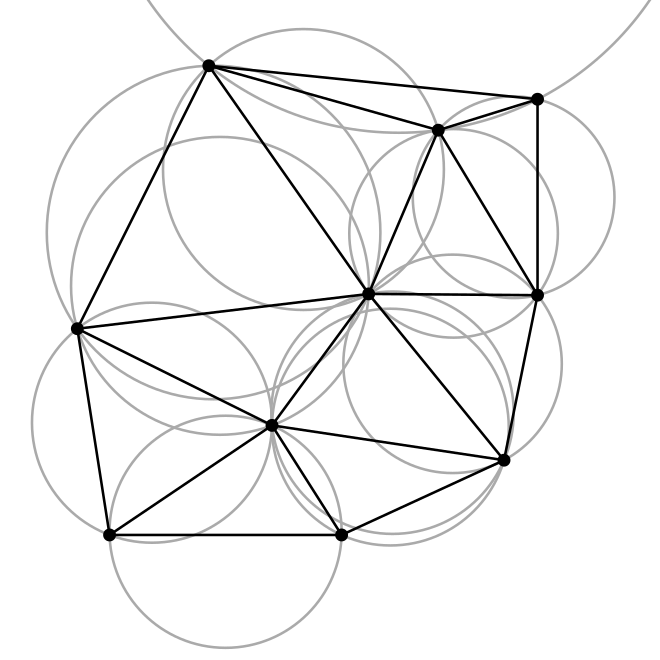
\includegraphics[width=2.5in]{images/illus_graphs/Delaunay_circumcircles_vectorial.svg.png}
    \caption{Example of a Delaunay triangulation}
    \label{del_tri}
\end{figure}

\subsection{Gabriel graph}
\noindent The Gabriel graph is a subgraph of a Delaunay triangulation. Thus, if the Delaunay triangulation is given, it can be found in a linear time. 

Gabriel graphs are named after K. Ruben Gabriel, who introduced them in a paper with Robert R. Sokal in 1969[citer].

Formally, it is the graph $G$ with vertex set $S$ in which any two distinct points $p\in S$ and $q\in S$ are adjacent precisely when the closed disc having pq as a diameter contains no other points.

\subsection{$k$-NN graph}
\noindent Nevertheless, the two methods presented above are triangulation, that is to say that they do not connect each \acrshort{bs} to all of its potential neighbours.

One simple idea to get rid of this problem could be solved by connecting each \acrshort{bs} to its $k$ nearest neighbours.

\section{Finding the real neighbours}

\noindent Each of the precedent methods gives us a list of potential neighbours for each \acrshort{bs}. However, we know that some of this neighbouring connexions are wrong,
because some \acrshort{bs} will be \og hidden\fg{} by others.

Thus, we need to find methods to suppress bad connexions. That was made by Delphine.

The main innovation of our work is to take in account the difference of \acrshort{bs}'s density.

\subsection{Measurement of \acrshort{bs} density}
\noindent To simplify the explanation, and because it is related, we will assume that solving this problem is equivalent to finding the \acrshort{bs} situated in \og cities\fg{}.

\subsubsection{DBScan}

\subsubsection{HDBScan}

\subsubsection{$3$-NN mean distance}
One provider $\gamma$

To classify each base station we need a method. Here, we will take the mean distance to the 3 nearest neighbours.

Let's call this value $\gamma$, in $\unit{km}$. So, we have 4 different categories.
For each category, we will apply a different distance and angle criterion :

\subsection{Filtering criteria}

\begin{table}[!b]
    \centering
    \caption{Summary of criteria values}
    \label{crit_summary}
    \begin{tabular}{clcc}
        \toprule
        \textbf{$\gamma$} & \textbf{Description} & \textbf{max\_distance} & \textbf{min\_angle} \\
        \cmidrule(lr){1-4}
        $\left[0, 1\right]$ & city center & $\unit[2]{km}$ & $5^\circ$ \\
        $\left]1, 2\right]$ & urban area & $\unit[5]{km}$ & $10^\circ$ \\
        $\left]2, 4\right]$ & extra-urban area & $\unit[10]{km}$ & $15^\circ$ \\
        $\left]4, \infty\right[$ & courntryside & $\unit[15]{km}$ & $20^\circ$ \\
        \bottomrule
    \end{tabular}
\end{table}

\begin{figure}[!t]
    \centering
    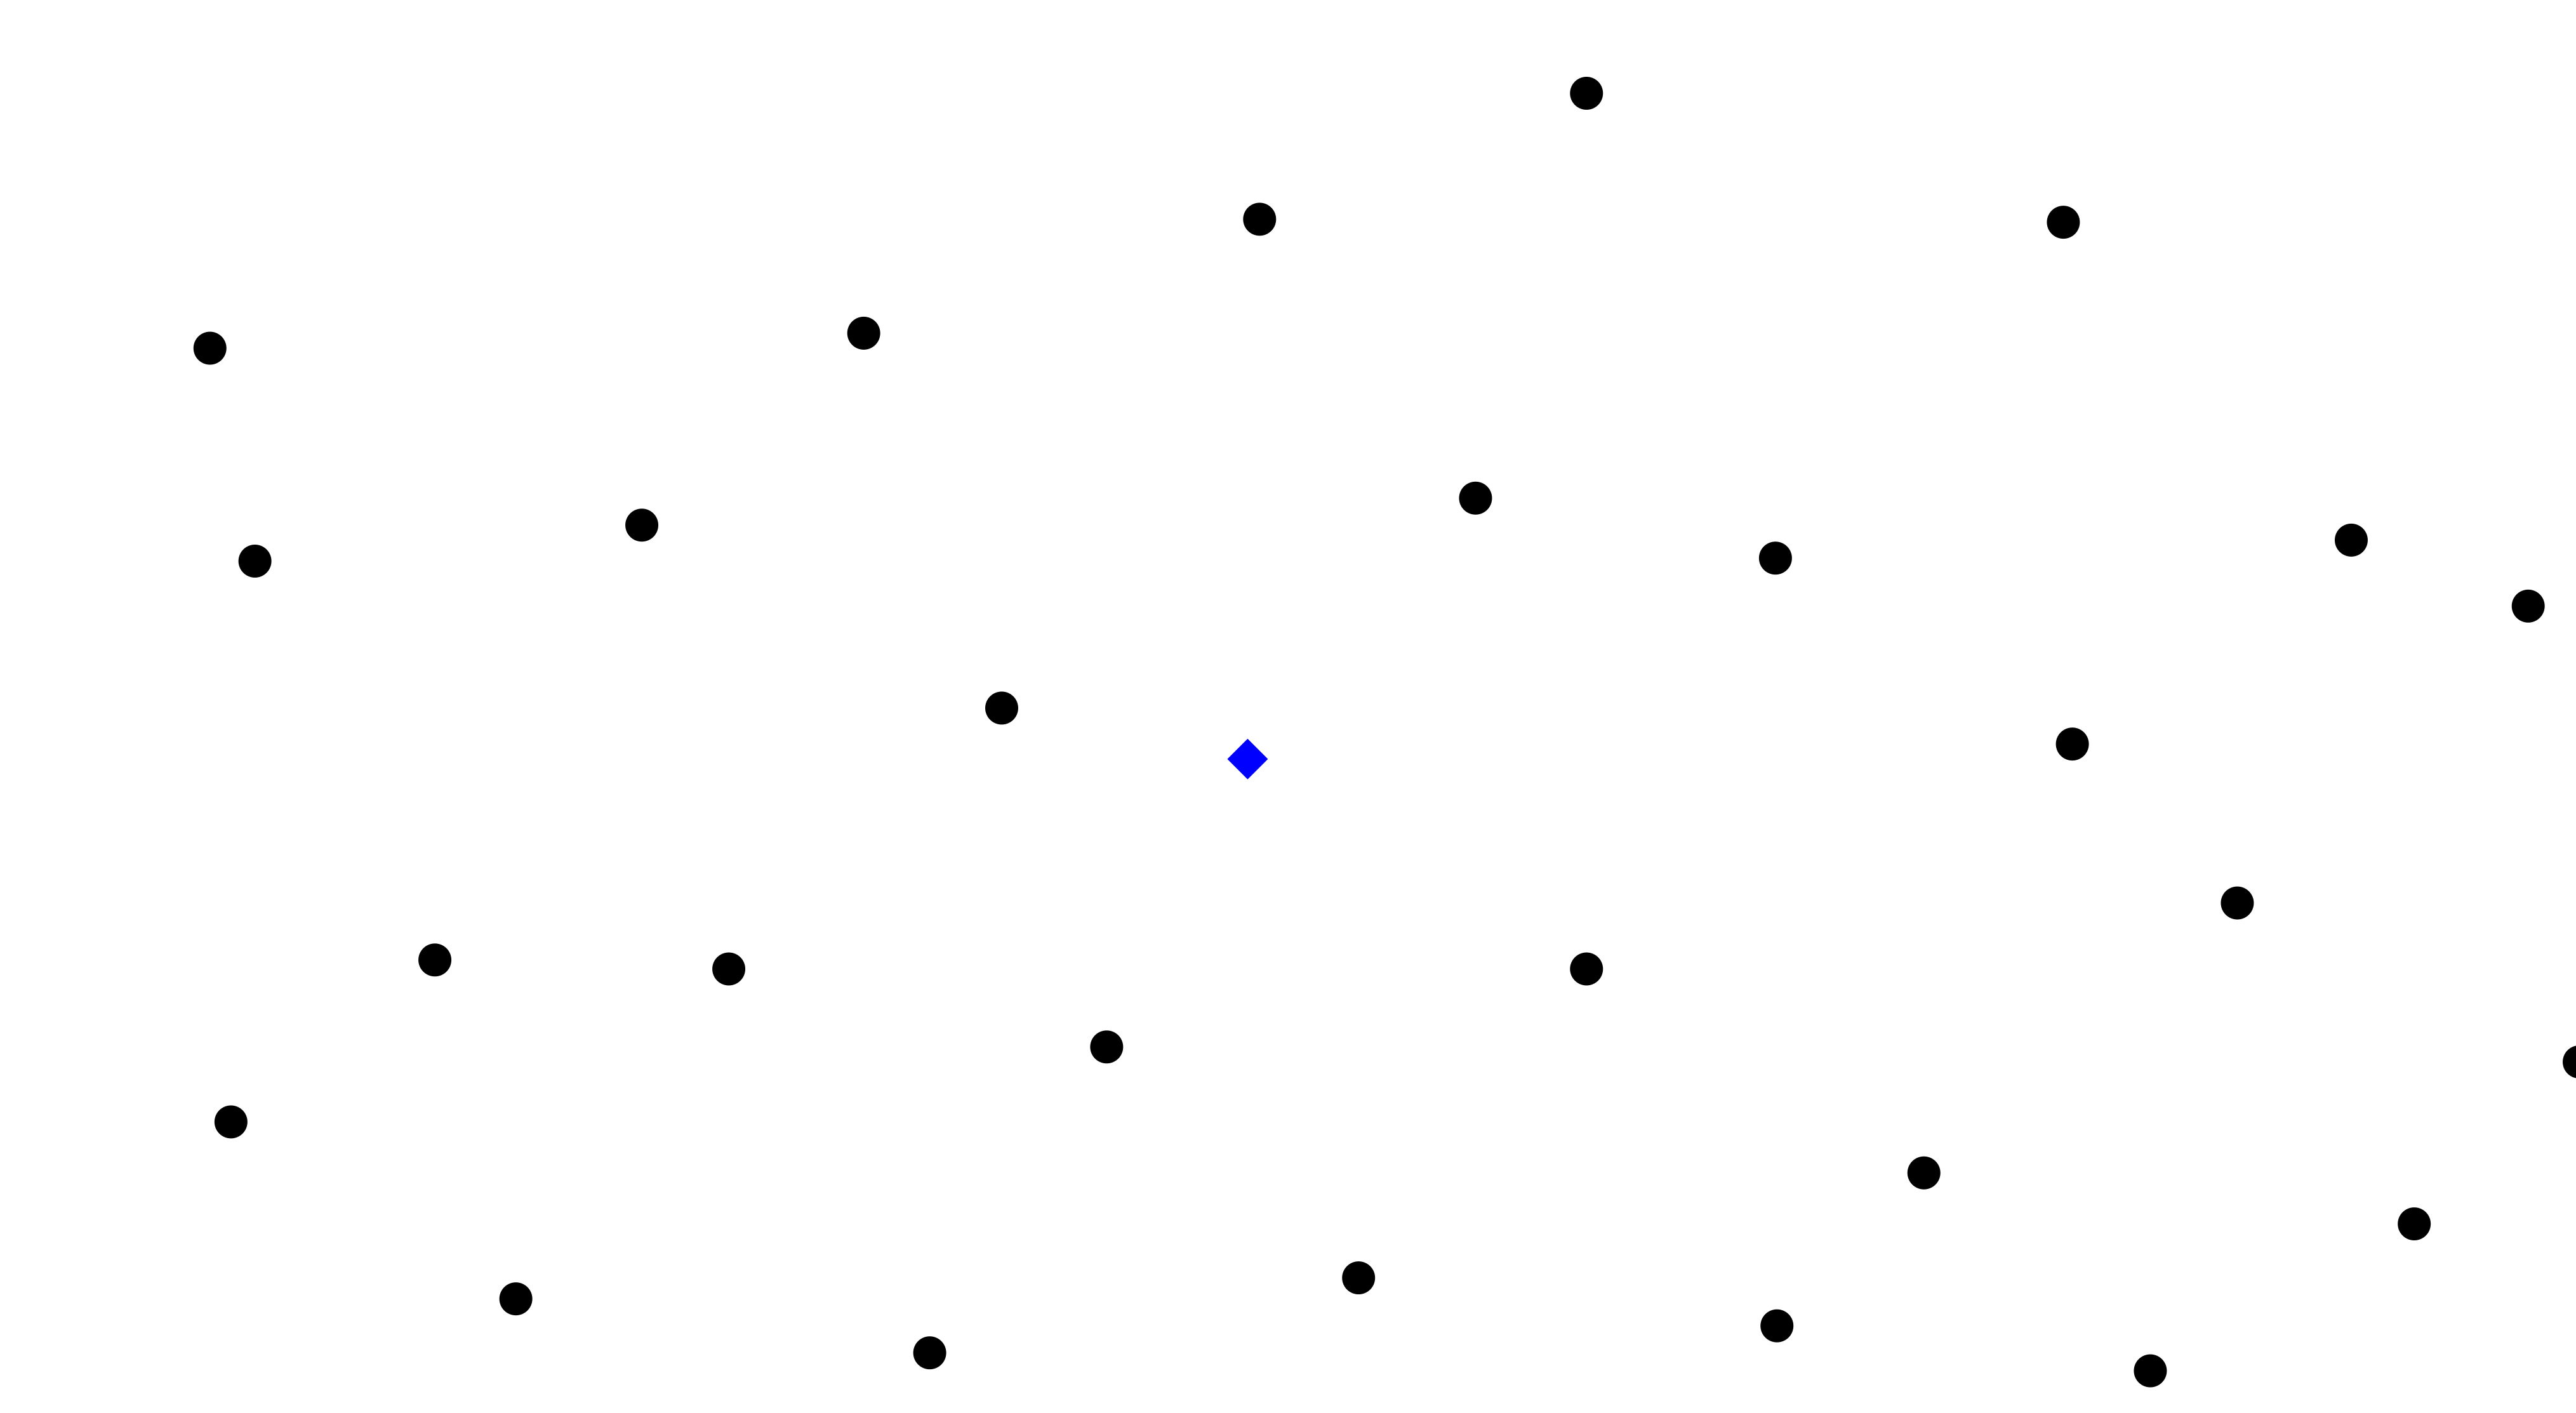
\includegraphics[width=2.5in]{images/illus_crit/points.png}
    \caption{Example of a Delaunay triangulation}
    \label{crit_pts}
\end{figure}

\begin{figure}[!b]
    \centering
    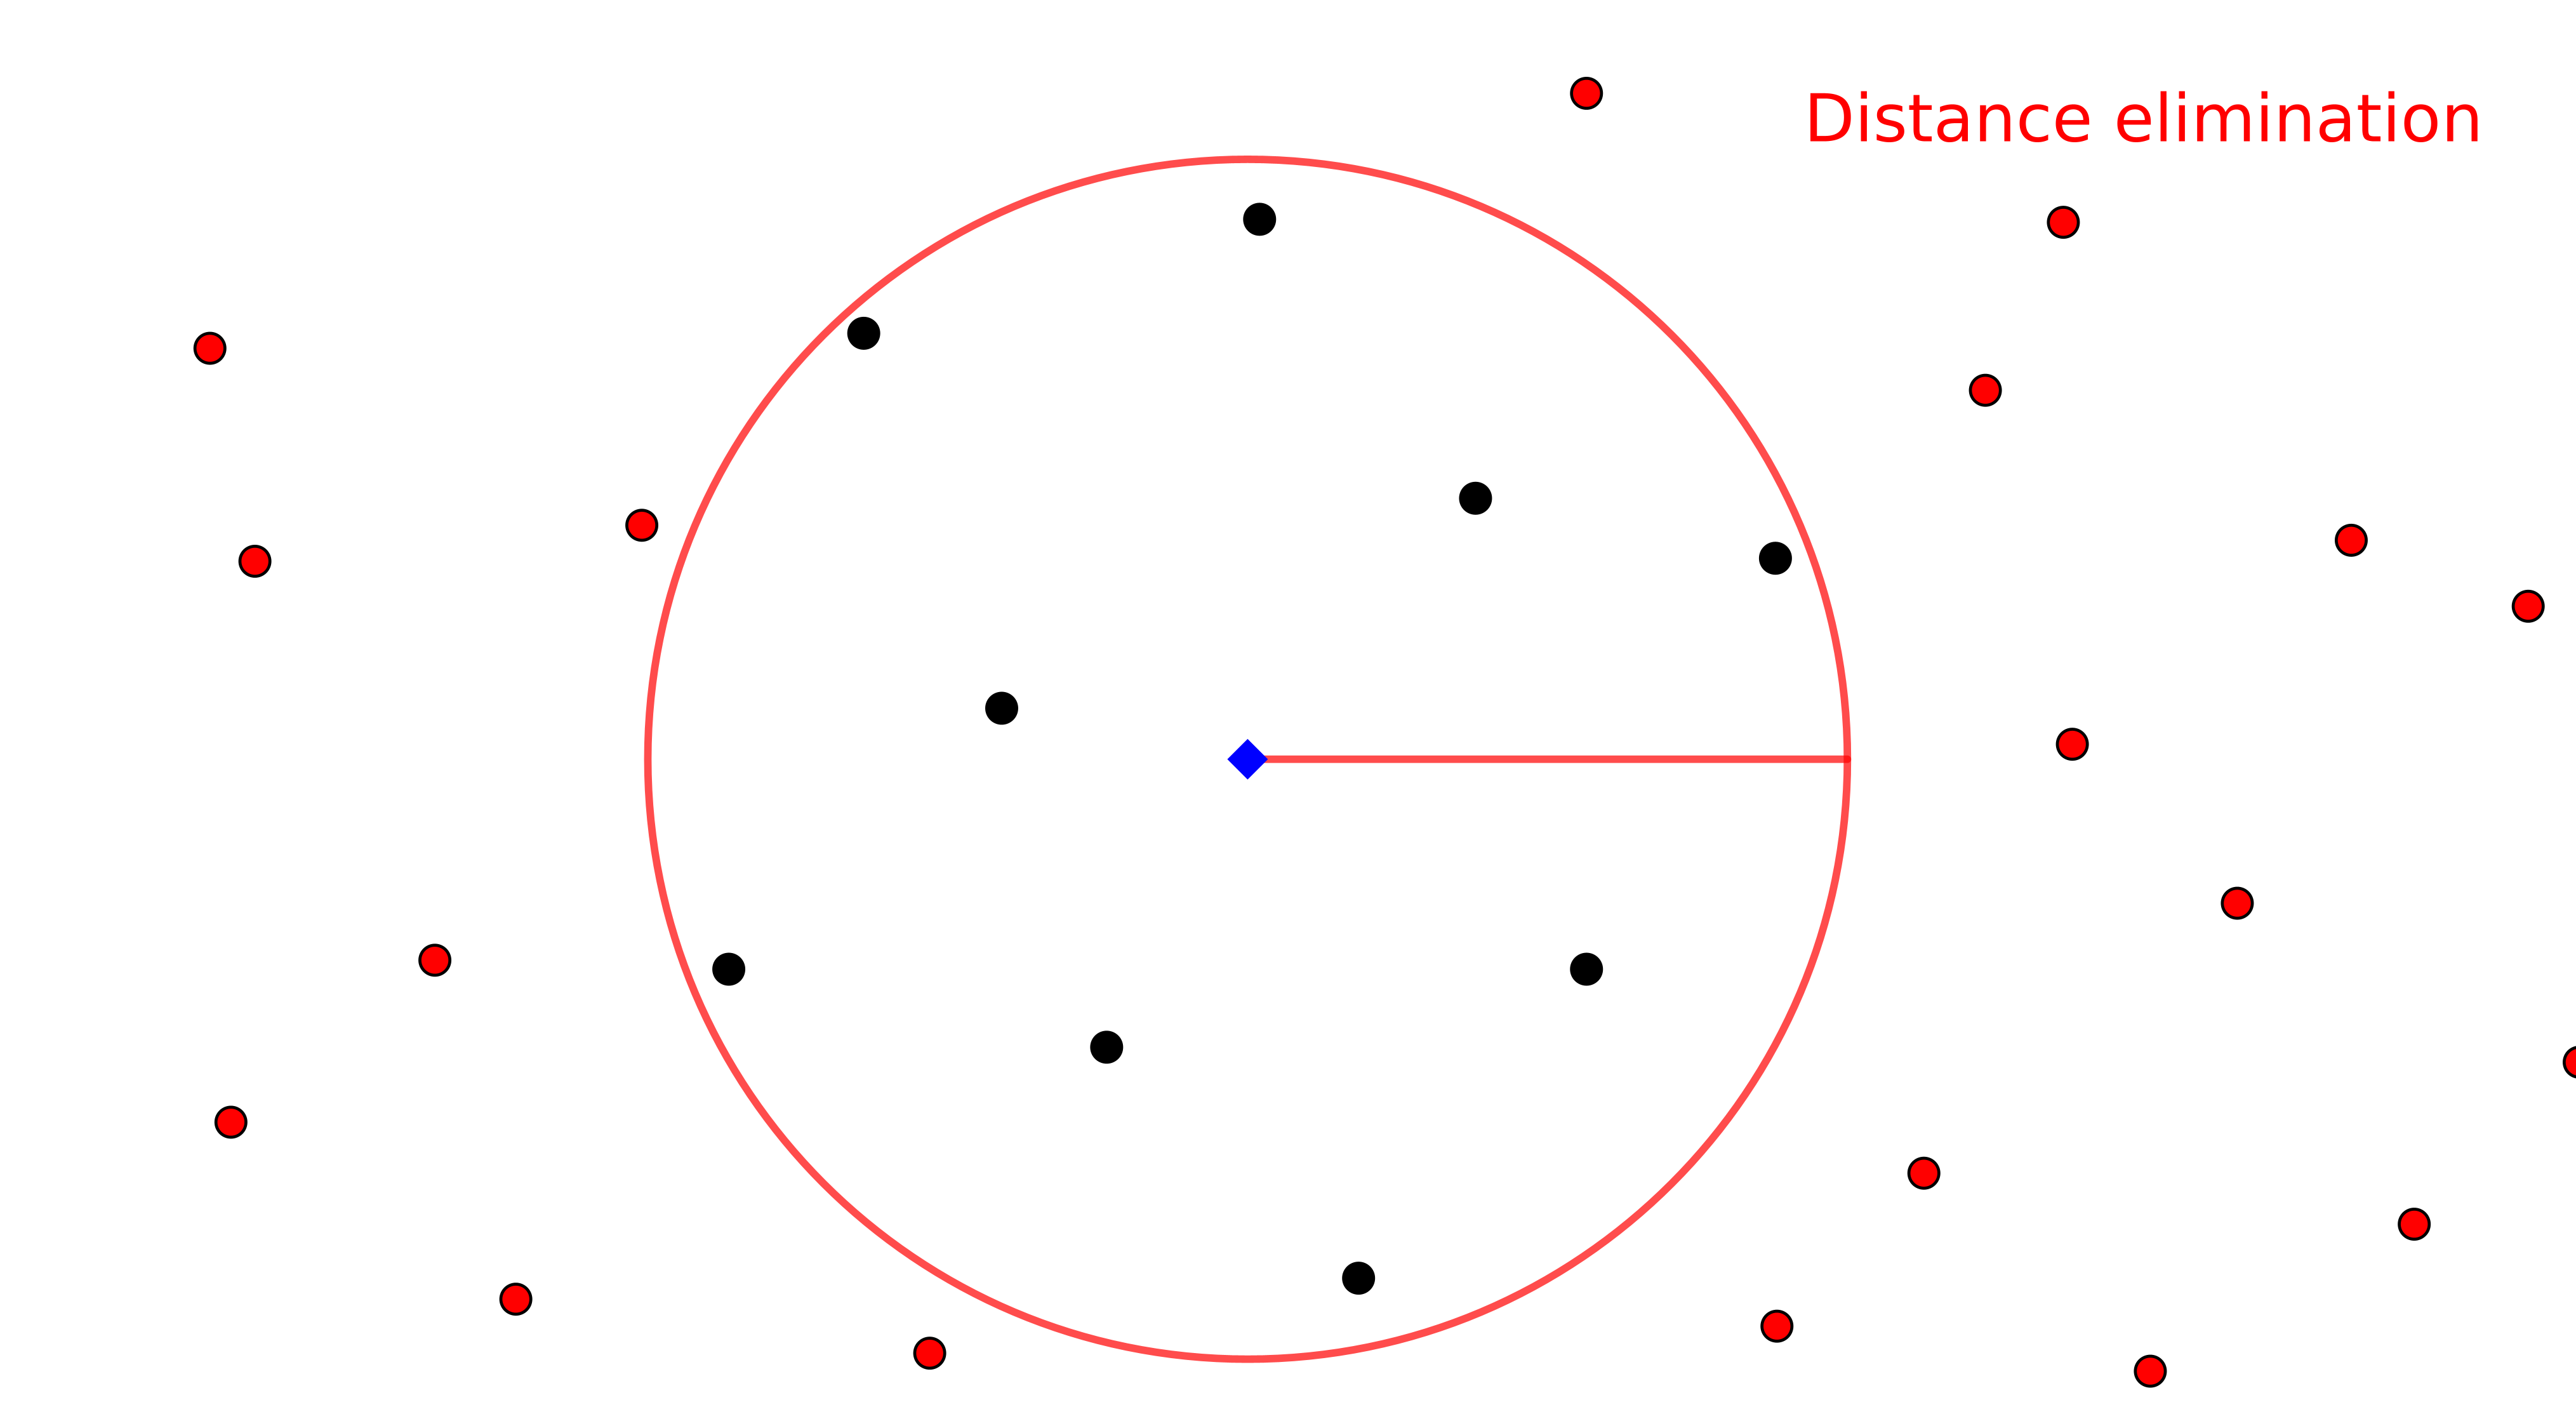
\includegraphics[width=2.5in]{images/illus_crit/distance_elim.png}
    \caption{Example of a Delaunay triangulation}
    \label{crit_dis}
\end{figure}

\begin{figure}[!t]
    \centering
    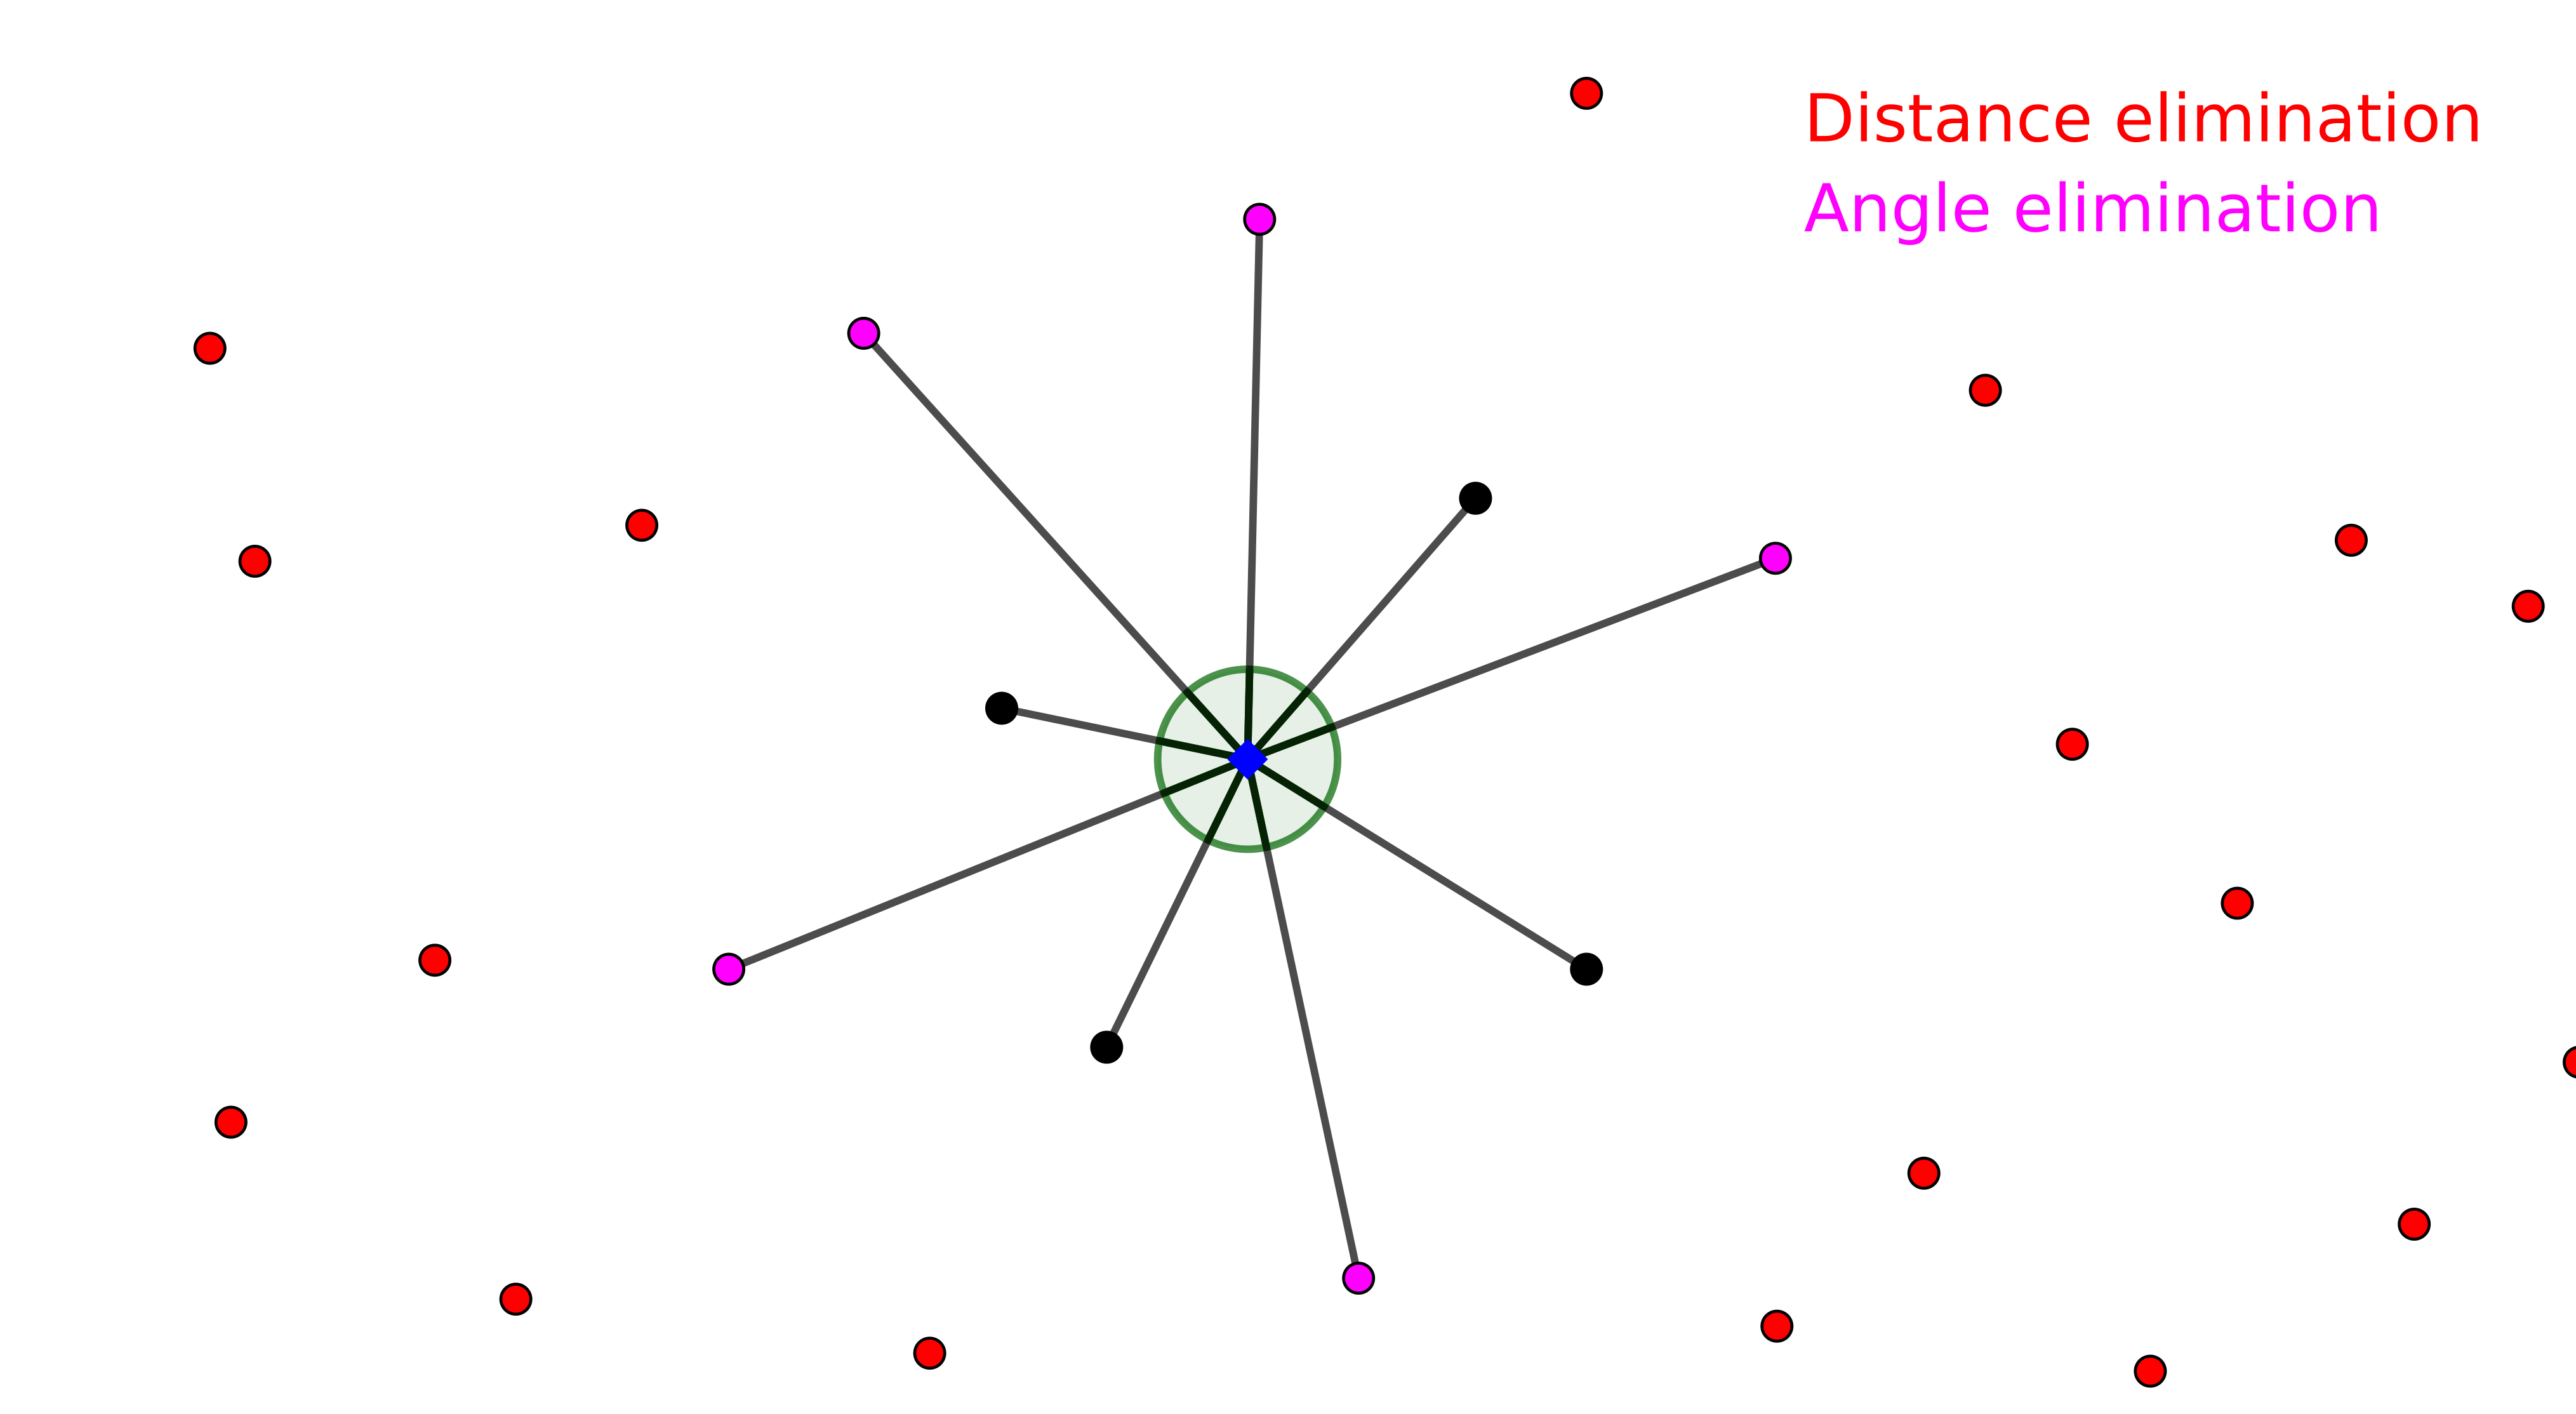
\includegraphics[width=2.5in]{images/illus_crit/angle_elim.png}
    \caption{Example of a Delaunay triangulation}
    \label{crit_ang}
\end{figure}

\begin{figure}[!b]
    \centering
    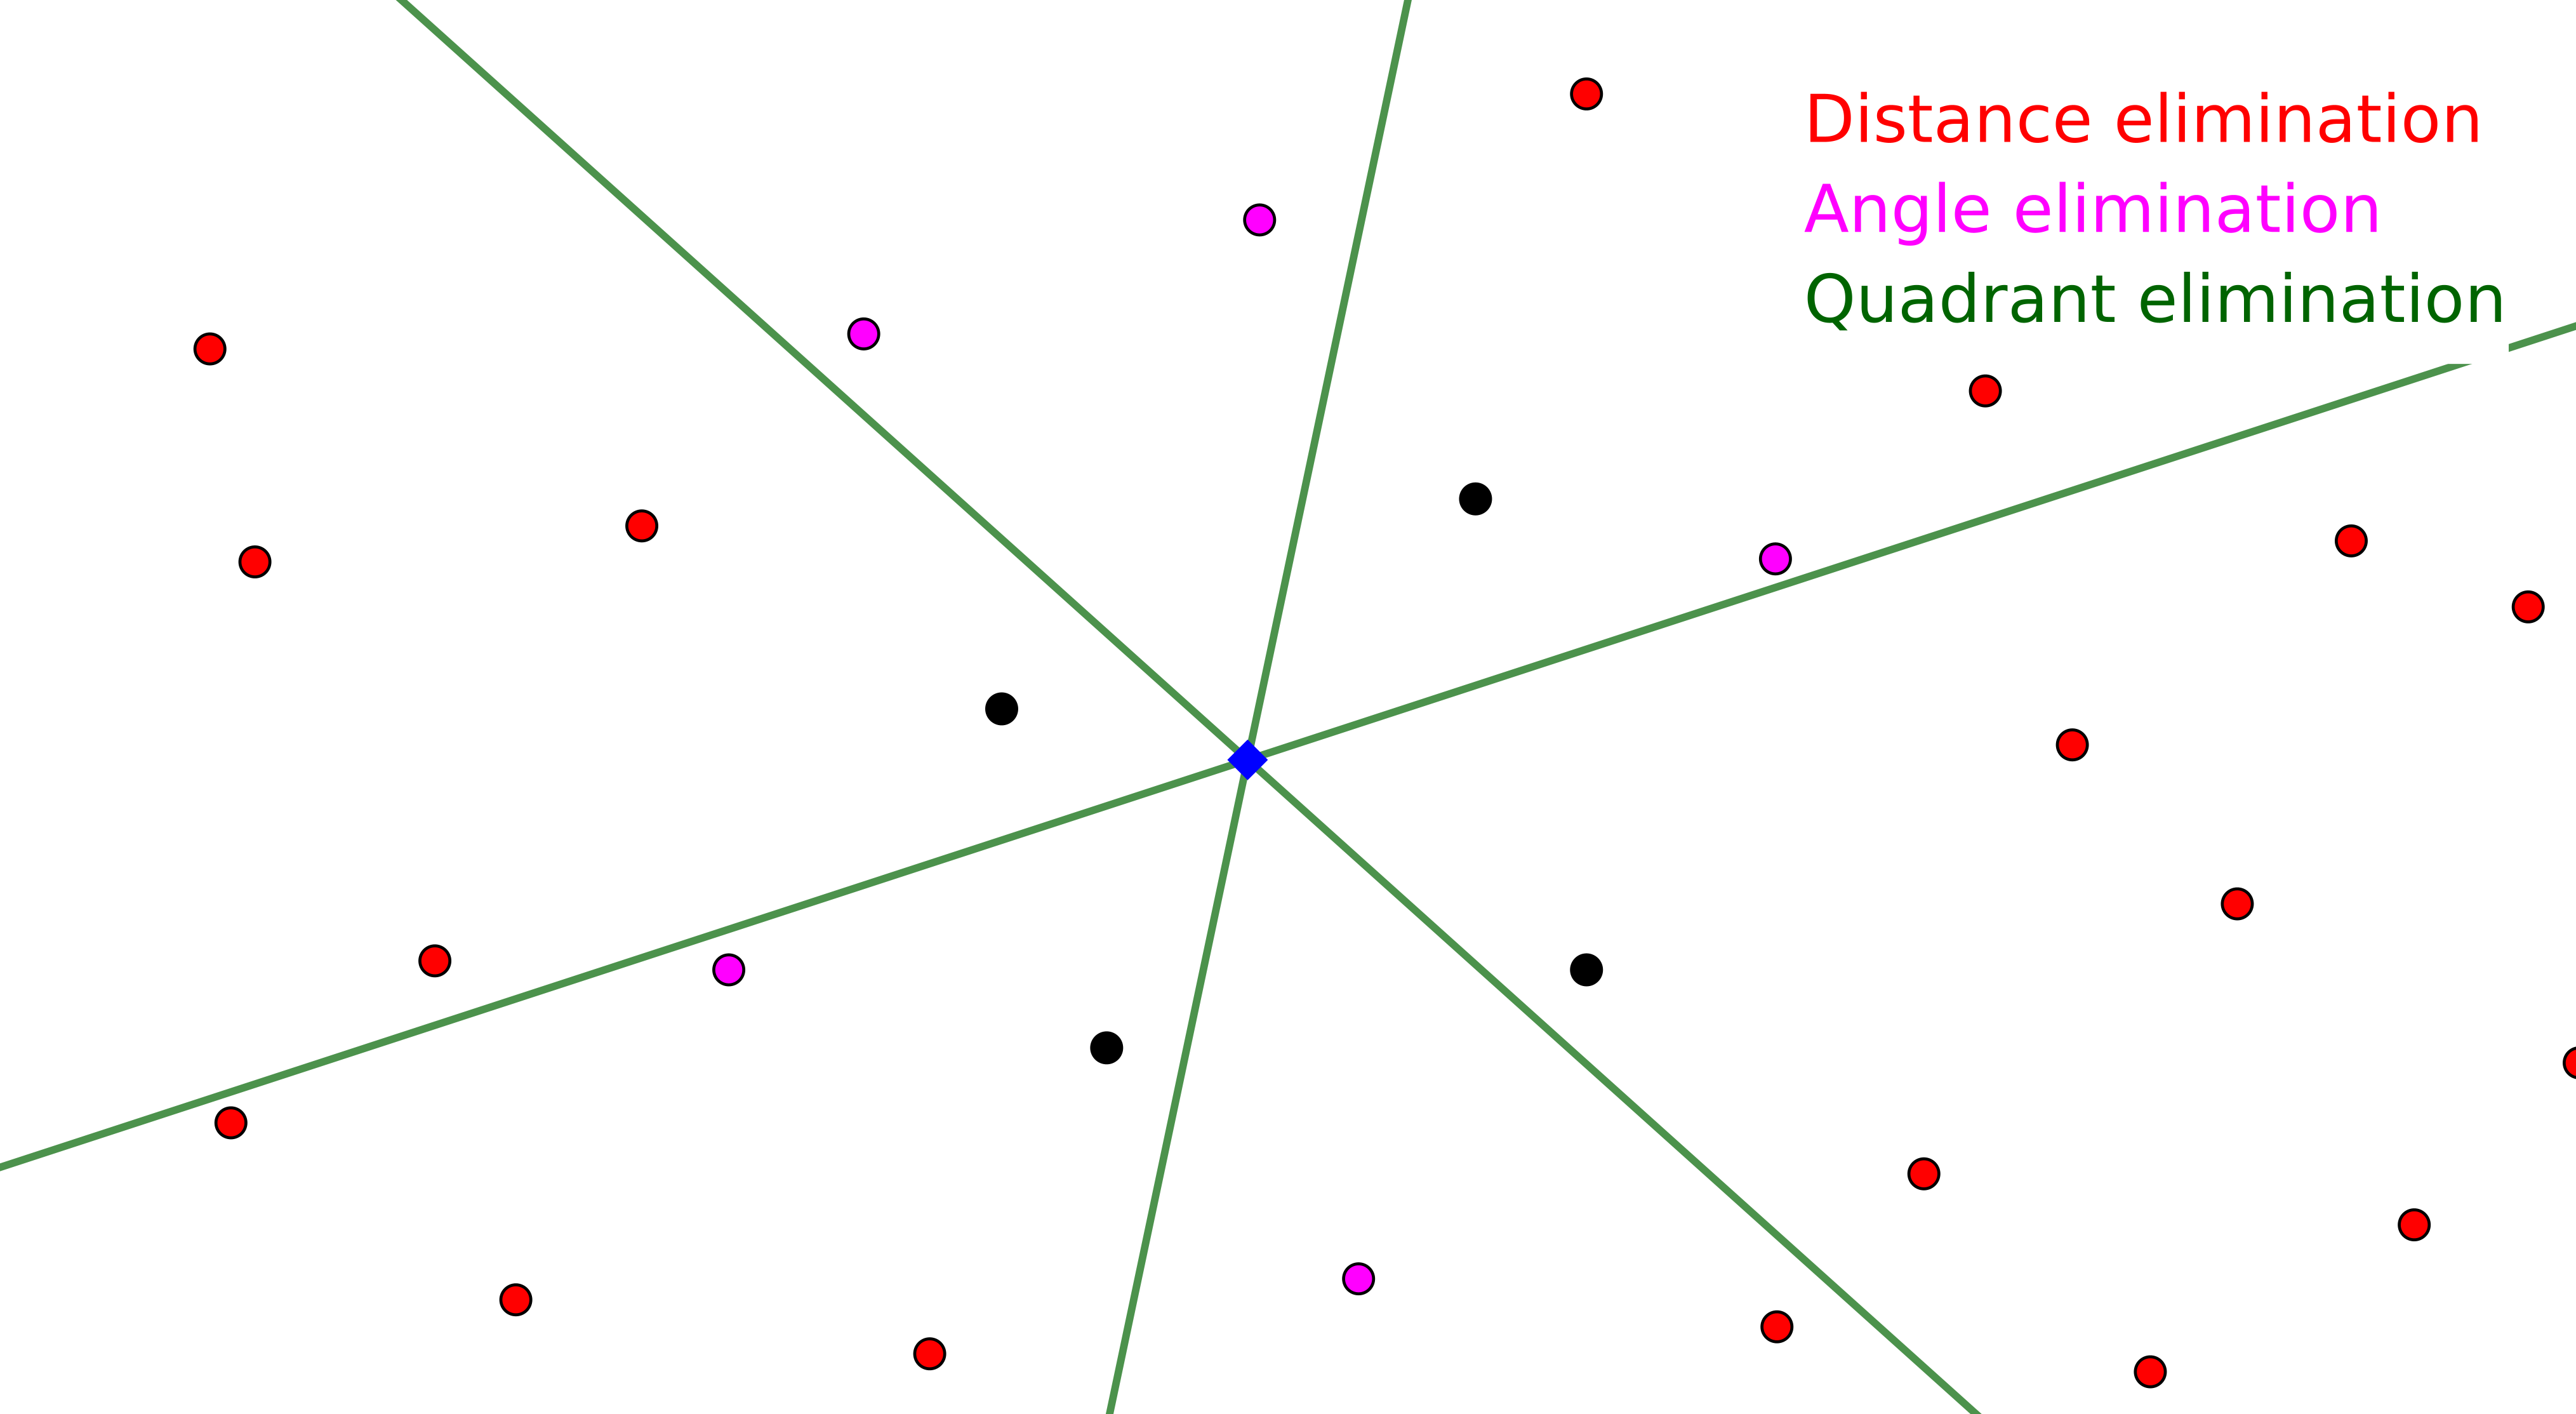
\includegraphics[width=2.5in]{images/illus_crit/quadrant_elim.png}
    \caption{Example of a Delaunay triangulation}
    \label{crit_qua}
\end{figure}

\begin{figure}[!t]
    \centering
    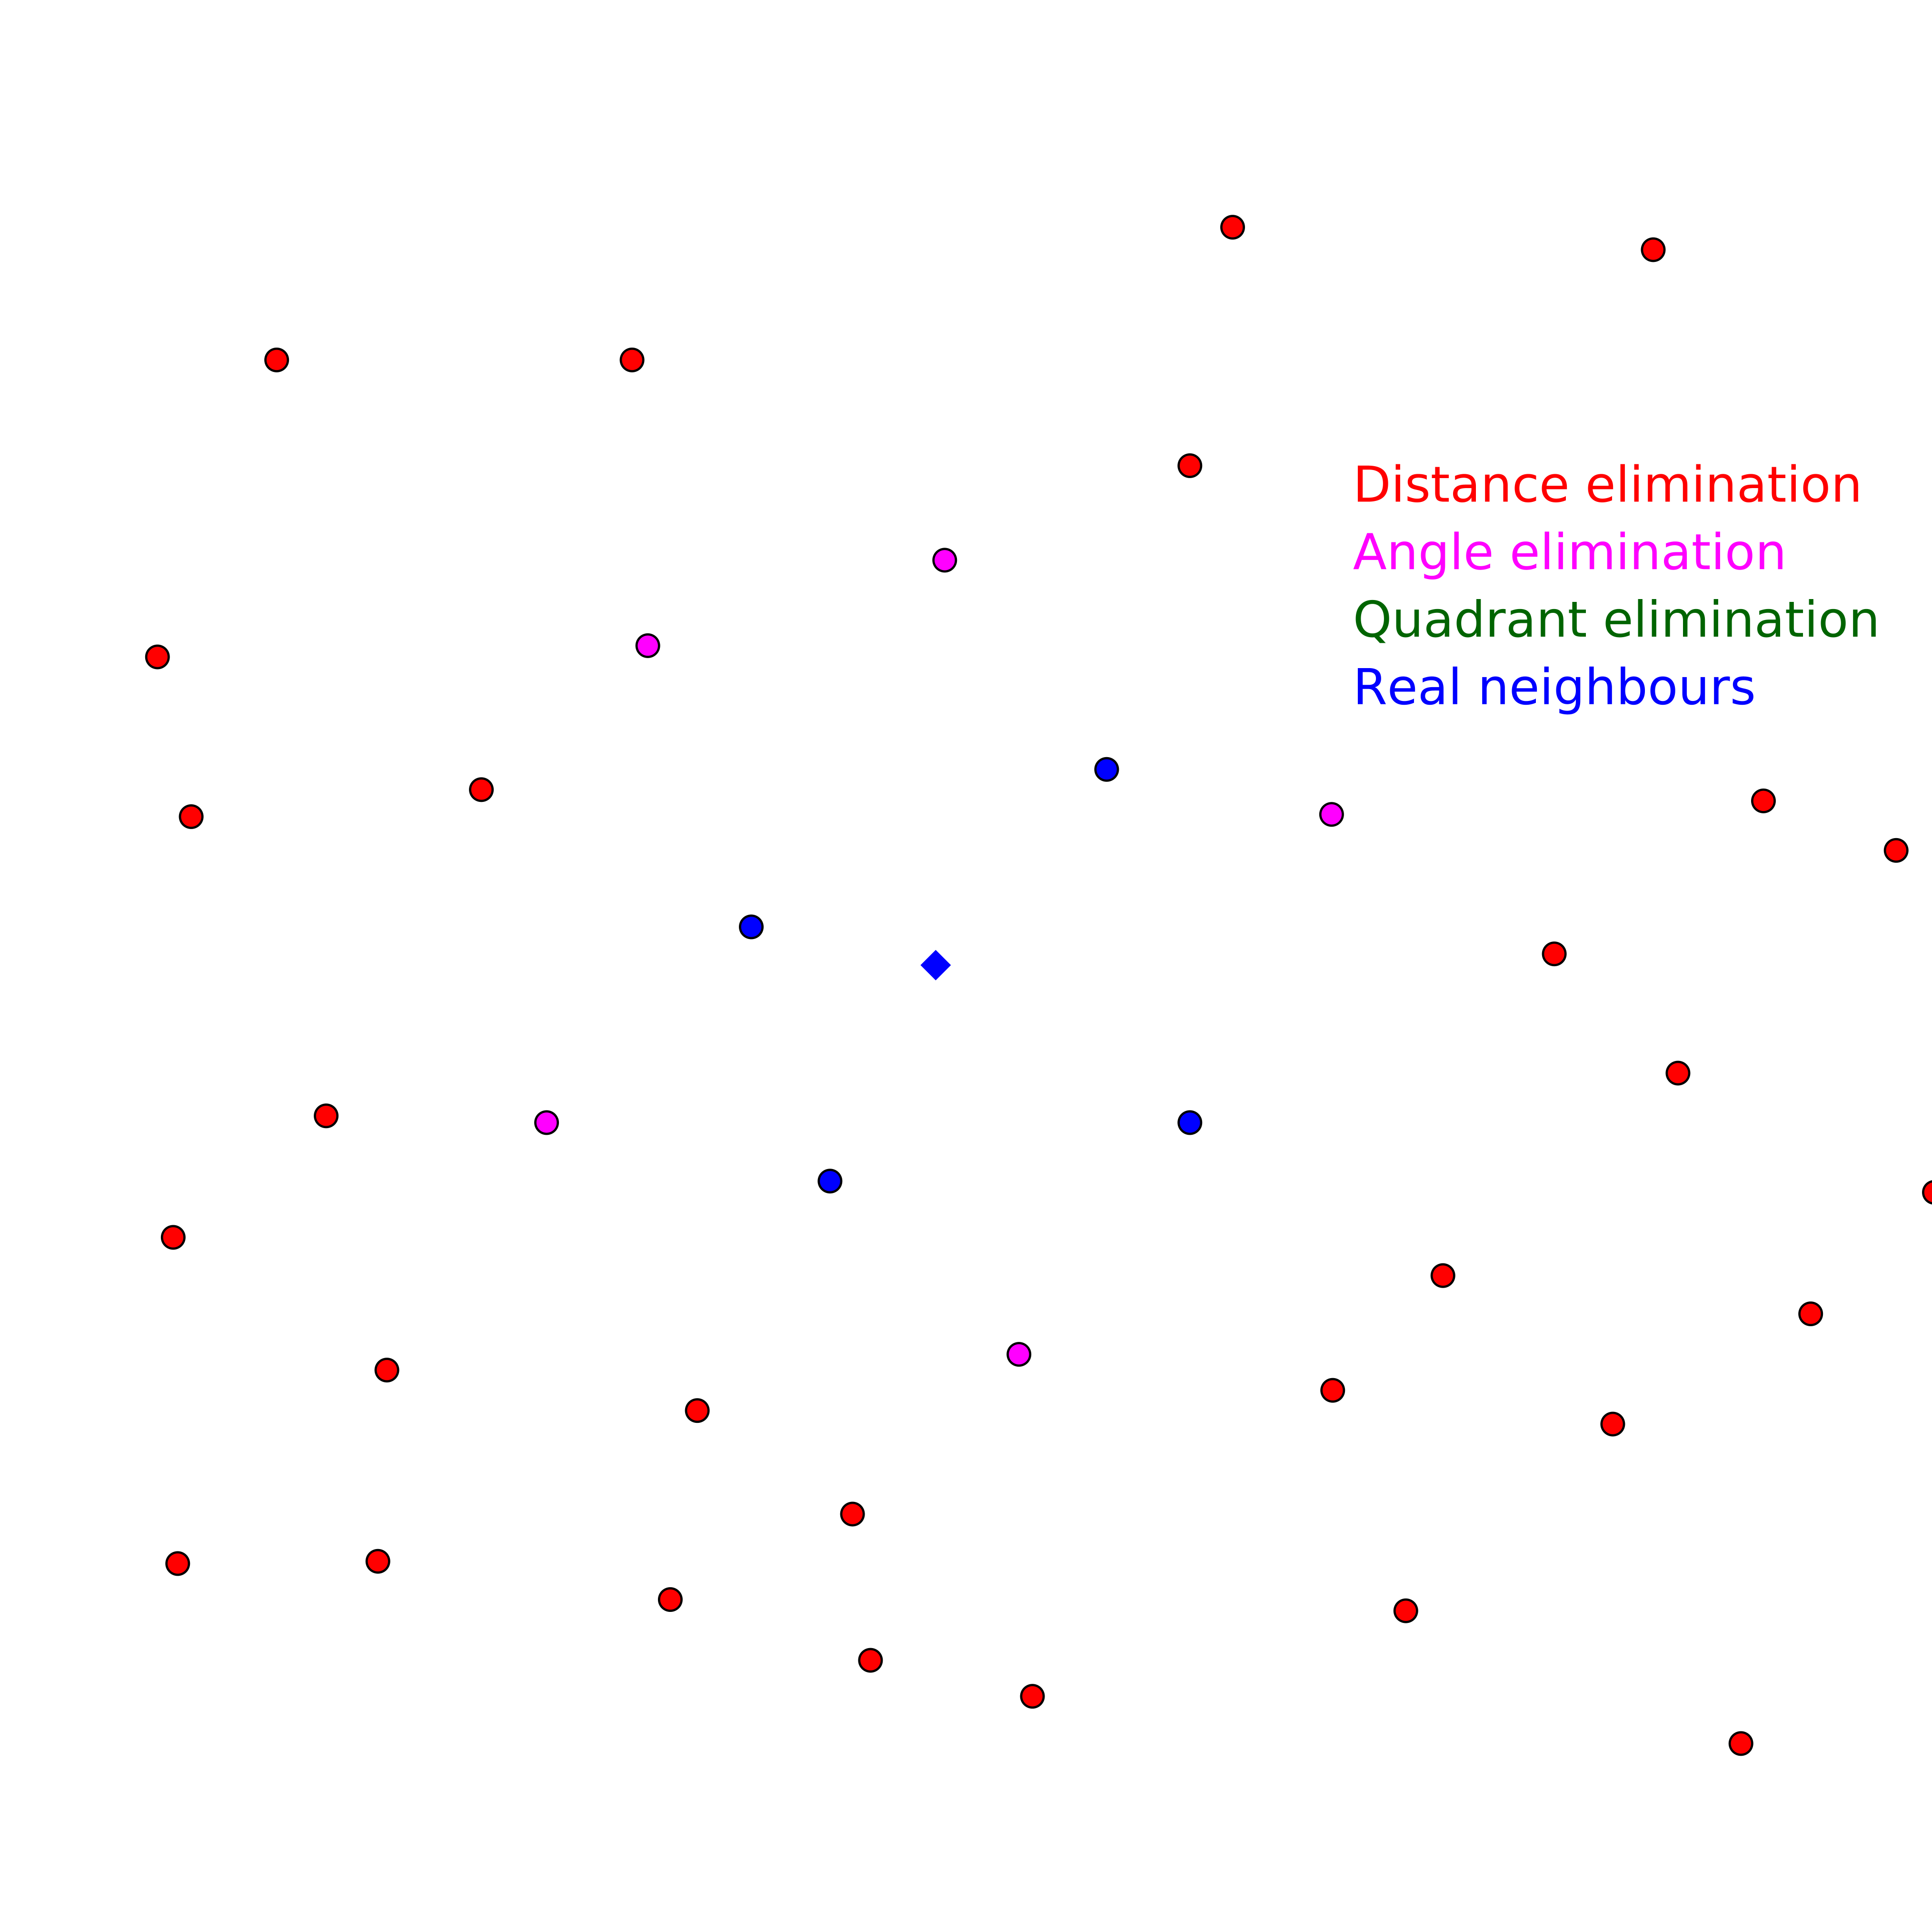
\includegraphics[width=2.5in]{images/illus_crit/neighs.png}
    \caption{Example of a Delaunay triangulation}
    \label{crit_nei}
\end{figure}

\subsubsection{Distance criterion}
Each \acrshort{bs} has its proper coverage area, which is not infinite. As a matter of fact, we need to suppress longer edges.

\subsubsection{Angle criterion}
For each \acrshort{bs}, we 

\subsubsection{Quadrant criterion}

\section{Results}

\section{Conclusion}

[Ouverture : prendre en compte les zazimuths]

\printglossary[type=\acronymtype]

\bibliographystyle{alpha}
\bibliography{./biblio.bib}

\end{document}


